%--------------------
% Packages
% -------------------
\documentclass[11pt,a4paper]{article}
\usepackage[utf8x]{inputenc}
\usepackage[T1]{fontenc}
%\usepackage{gentium}
\usepackage{mathptmx} % Use Times Font


\usepackage[pdftex]{graphicx} % Required for including pictures
\usepackage[pdftex,linkcolor=black,pdfborder={0 0 0}]{hyperref} % Format links for pdf
\usepackage{calc} % To reset the counter in the document after title page
\usepackage{enumitem} % Includes lists
\usepackage{dirtree}
\usepackage{listings}
\usepackage{jupynotex}
\usepackage{minted}

\lstset{
    basicstyle=\ttfamily,
    breaklines=true,
}


\frenchspacing % No double spacing between sentences
\linespread{1.2} % Set linespace
\usepackage[a4paper, lmargin=0.1666\paperwidth, rmargin=0.1666\paperwidth, tmargin=0.1111\paperheight, bmargin=0.1111\paperheight]{geometry} %margins
%\usepackage{parskip}

\usepackage[all]{nowidow} % Tries to remove widows
\usepackage[protrusion=true,expansion=true]{microtype} % Improves typography, load after fontpackage is selected


%-----------------------
% Set pdf information and add title, fill in the fields
%-----------------------
\hypersetup{ 	
pdfsubject = {Research Computing Coursework},
pdftitle = {Research Computing Coursework},
pdfauthor = {Laura Just Fung (lj441)}
}

%-----------------------
% Begin document
%-----------------------
\begin{document} 

\section{Introduction}
This report discusses development of the package designed to implement automatic differentiation using dual numbers in Python. 

Dual numbers are an extension of real numbers, typically used for automatic differentiation in areas such as research computing and machine learning.

A dual number is defined like so:

\begin{equation}
    \mathrm{Dual} = a + b \epsilon
\end{equation}

Where $a$ represents the real part, and $b\epsilon$ represents the dual part. $a$ and $b$ are real numbers, and $\epsilon$ represents an infinitesimally small number such that $\epsilon^2 = 0$ but $\epsilon \neq 0$.

Their utility lies in the fact that a dual number automatically encodes the differentiation of the real part in the dual part. This makes them especially useful in machine learning, where derivatives are frequently calculated but can be expensive to obtain.

\section{Repository}
\subsection{Structure}
Good practice suggests the following directory structure:

\dirtree{%
.1 dual{\_}autodiff.
.2 report.
.3 \ldots.
.2 dual{\_}autodiff.
.3 {\_}{\_}init{\_}{\_}.py.
.3 dual.py.
.2 tests.
.3 test{\_}dual.py.
.2 docs.
.3 \ldots.
.2 build.
.3 \ldots.
.2 source.
.3 \ldots
.2 pyproject.toml.
.2 setup.py.
.2 README.md.
.2 Makefile.
.2 LICENSE.
}

\subsection{Project configuration}
In order to compile this package, a \texttt{pyproject.toml} file was used. The following is its contents:
\lstinputlisting[caption={pyproject.toml}]{../pyproject.toml}

\section{Implementation}
In order to create a package that implements dual numbers, a class that defines what a dual number is must first be created. Afterwards, the usual binary operations (addition, subtraction, multiplication, division, exponentiation, etc.) in Python are overloaded with the dual implementations. After that, additional functions can be overloaded, including \texttt{NumPy} and \texttt{mpmath} trigonometric functions, so that dual numbers can be handled as well as real numbers. 
\subsection{Dual class}
The \texttt{Dual} class is defined and initialised like so:
\lstinputlisting[caption={Dual class},language=python,linerange={5,14,22, 23}]{../dual_autodiff/dual.py}
The \texttt{real} and \texttt{dual} variables are defined as attributes of the \texttt{Dual} class that can be accessed publicly.

A dual number can be initialised as follows:
\jupynotex[2]{../dual_autodiff.ipynb}
And it produces the following output when printed:
\jupynotex[3]{../dual_autodiff.ipynb}
\subsection{Binary operations}
Binary operations include: addition, subtraction, multiplication, division, and exponentiation. The \texttt{Dual} class allows for these operations to performed over dual numbers as well as real numbers when overloaded.
An example is as follows:
\jupynotex[4]{../dual_autodiff.ipynb}
\subsection{Unary operations}
The unary operations implemented in the Dual class include trigonometric functions (sine, cosine, tangent), inverse trigonometric functions, hyperbolic functions, some inverse hyperbolic functions, the natural logarithm function, and the exponential function.
An sample of the functions implemented is shown below:
\jupynotex[5]{../dual_autodiff.ipynb}

\subsection{Collections}


\section{Local package}
The Python package is installable with \texttt{pip install -e .} from the root project folder \texttt{dual\_autodiff}. The package is importable with \texttt{import dual\_autodf as df}.

\section{Differentiation}
Consider the function
\begin{equation}
    f(x) = \log{\sin{x}} + x^2 \cos{x}
    \label{eq:func}
\end{equation}

where $x=1.5$. The derivative can be easily calculated using \texttt{dual\_autodiff}:
\jupynotex[6]{../dual_autodiff.ipynb}

Comparing this to the analytic result

\begin{equation}
    \frac{df}{dx} = \frac{\cos{x}}{\sin{x}} + 2 x \cos{x} - x^2 \sin{x} 
\end{equation}

and various numerical methods including the central

\begin{equation}
    \frac{d}{dx} f(x) \approx \frac{f(x+h) - f(x-h)}{2h},
\end{equation}

forward

\begin{equation}
    \frac{d}{dx} f(x) \approx \frac{f(x+h) - f(x)}{2h},
\end{equation}

backward

\begin{equation}
    \frac{d}{dx} f(x) \approx \frac{f(x) - f(x-h)}{2h},
\end{equation}

and five-point equations

\begin{equation}
    \frac{d}{dx} f(x) \approx \frac{-f(x+2h) + 8 f(x+h) - 8 f(x-h) + f(x-2h)}{12h},
\end{equation}

where accuracy mostly depends on the step size $h$. For the following comparisons in Table~\ref{tab:diffs}, a step-size of $h=1 \times 10^{-5}$ was used.

\begin{table}
    \centering
    \begin{tabular}{c|c|c}
        Method & Result (12 d.p.) & Percentage difference (\%) (12 d.p.)\\
        \hline
        \texttt{Dual} & -1.961237270553 & $0.0$\\
        Analytic & -1.961237270553 & $0.0$\\
        \hline
        Central & -1.961237270641 & $4.466\times 10^{-9}$\\
        Forward & -1.961272309059 & $1.786551078000\times 10^{-3}$\\
        Backward & -1.961202232223 & $1.786542145000 \times 10^{-3}$\\
        Five-point & -1.96123727058 & $1.353\times 10^{-9}$\\
        \hline
        Richardson central & -1.961237270561 & $4.1\times 10^{-10}$\\
        Richardson forward & -1.961248950033 & $5.955158990000\times 10^{-4}$\\
        Richardson backward & -1.961225591090 & $5.955150808000\times 10^{-4}$\\
        Richardson five-point & -1.961237270558 & $2.21\times 10^{-10}$
    \end{tabular}
    \caption{Results of each method and percentage difference of each from the \texttt{Dual} result.}
    \label{tab:diffs}
\end{table}



The Richardson extrapolation was also used to improve the accuracy of the numerical methods. It works by taking two central approximations of the differentiation with two different step sizes $h$ and $\frac{h}{2}$ and using these to eliminate the $O(h^2)$ error term:

\begin{equation}
    D(h) = \frac{f(x+h) - f(x-h)}{2h}, 
\end{equation}

\begin{equation}
    D\biggl(\frac{h}{2}\biggr) = \frac{f(x+\frac{h}{2}) - f(x-\frac{h}{2})}{h}, 
\end{equation}

\begin{equation}
    \frac{d}{dx} f(x) \approx \frac{4 D(\frac{h}{2}) - D(h)}{3}.
\end{equation}

Comparing the numerical methods to the \texttt{Dual} result, it can be seen that with increasing step size $h$, the percentage difference gets larger, as shown in Fig.~\ref{fig:pdiff}.

\begin{figure}
    \centering
    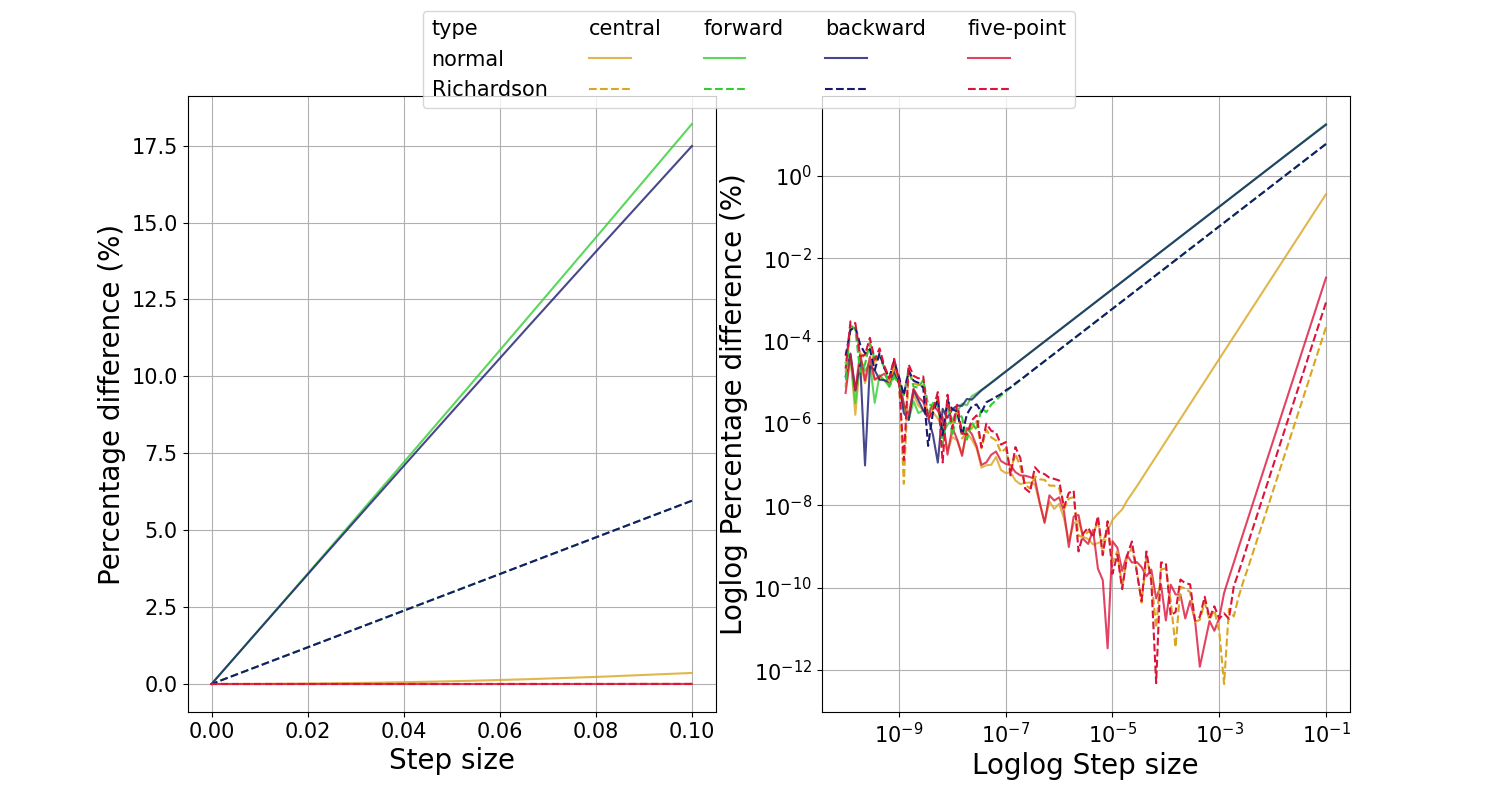
\includegraphics[width=\columnwidth, keepaspectratio]{../percentage_difference.png}
    \caption{Percentage difference between numerical and \texttt{Dual} results for the differentiation of Eq.~\ref{eq:func} at $x=1.5$ as a function of step-size $h$.}
    \label{fig:pdiff}
\end{figure}

\section{Test suite}
Test suites for each of the overloaded operations and functions were made in \texttt{test\_dual.py}.

Tests were made for both left and right-sided operations, ensuring that the \texttt{Dual} class can operate on and be operated on by both real and Dual numbers. Tests were also made for the unary functions to ensure that the correct differentiation of each function was made.

Additional tests were also made for the Cythonised \texttt{Dual} class, to show that there is no decrease in functional performance.

Tests can be run using \texttt{python -m pytest tests} from within the root directory.

\section{Project documentation with \texttt{\textbf{Sphinx}}}
Project documentation was done using docstrings in the \texttt{dual.py} file and compiled with \texttt{Sphinx}. The documentation can be found in \texttt{docs}.

\section{Cythonization}
Cythonization is when a Python file is compiled into optimised C/C++. This allows for fast program execution and the ability to directly call C libraries. It uses \texttt{Cython} to do this, which requires either a \texttt{.py} or \texttt{.pyx} file to Cythonize.

Within the file, it is helpful to add \texttt{cdef} before any definitions of classes or functions and to also publicly declare any variables that need to be accessed outside of the class through \texttt{cython.declare(cython.float, visibility="public")}.

Then, using a \texttt{setup.py} file, \texttt{Cython} can be called to cythonize the program. An example of this can be seen below:

\lstinputlisting[caption={setup.py}]{../dual_autodiff_x/setup.py}

\section{Comparison between Cythonized and pure Python programs}

% The effects of Cythonization can be seen in Fig.~\ref{fig:memdiff} and Fig.~\ref{fig:timediff}. In terms of memory usage, the Cythonized \texttt{dual\_autodiff\_x} is much more efficient, while the pure Python \texttt{dual\_autodiff} takes up a lot more space.

In terms of time taken, \texttt{dual\_autodiff\_x} and \texttt{dual\_autodiff} tend to take about the same amount of time to execute operations. The main difference is that \texttt{dual\_autodiff\_x} tends to be a lot more stable, whilst \texttt{dual\_autodiff} exhibits intermittent spikes of lag.

The operations in which \texttt{dual\_autodiff\_x} shows the greatest performance boost are INSERT TEXT HERE.

For both \texttt{pow} and \texttt{exp} operations tend to take a lot of time, which is to be expected.

% \begin{figure}
%     \centering
%     \includegraphics[width=\columnwidth, keepaspectratio]{../mem_diff.png}
%     \caption{Performance of the Cythonized and pure Python versions of the \texttt{dual\_autodiff} functions in terms of memory usage.}
%     \label{fig:memdiff}
% \end{figure}

% \begin{figure}
%     \centering
%     \includegraphics[width=\columnwidth, keepaspectratio]{../time_diff.png}
%     \caption{Performance of the Cythonized and pure Python versions of the \texttt{dual\_autodiff} functions in terms of time taken.}
%     \label{fig:timediff}
% \end{figure}

\section{Wheels}

cibuildwheel is a package that uses Docker to create wheels specifically for different operating systems and architectures. Wheels are a way to distribute Python packages.

For this \texttt{dual\_autodiff\_x}, two wheels were created: one for Python 3.10 in a Linux x86 64 environment, and the other for Python 3.11 in the same environment.

These wheels can be found in \texttt{dual\_autodiff\_x/wheelhouse}.


\end{document}
